\begin{figure}[htbp]
\begin{subfigure}{0.72\textwidth}
    \begin{tikzpicture}
    [x=0.06667\textwidth, y=0.0667\textwidth]
    \draw (0,0) rectangle (15,7);
    % chamber
    \draw[fill=vacuum]
        (.5,1.5) rectangle (3.5,6.5);
    \draw[fill=gold]
        (1.7,1.95)--
        (2.3,1.95)--
        (2.3,1.8)--
        (1.7,1.8)--
        (1.7,1.95);
    \draw[fill=darkgrey]
        (1,2.1)--
        (1.65,2.1)--
        (1.75,1.8)--
        (2.25,1.8)--
        (2.35,2.1)--
        (3,2.1)--
        (3,2)--
        (2.4,2)--
        (2.3,1.7)--
        (1.7,1.7)--
        (1.6,2)--
        (1,2)--
        (1,2.1);
    \draw[gold,dashed,line width=0.003\textwidth]
        (2,2) -- (2,5);
    \coordinate (a) at (2,5);
    \def\theta{30}
    \draw[fill=darkgrey,rotate=\theta,shift={(a)}]
        (-1,-.1) rectangle (1,.1);
    \draw[angle,dotted,line width=0.003\textwidth,rotate=\theta,shift={(a)}]
        (0,-.1) -- (0,-1.5);
    \draw[angle,line width=0.002\textwidth,shift={(a)}]
        (0,-1.2) arc(270:270+\theta:1.2);
    \draw[fill=substrate,rotate=\theta,shift={(a)}]
        (-.2,-.1) rectangle (.2,.-.2)
        (-.8,-.1) rectangle (-.4,.-.2)
        (.4,-.1) rectangle (.8,.-.2);
    \draw[fill=sphere,rotate=\theta,shift={(a)}]
        (-.2,-.2) rectangle (.2,.-.22)
        (-.8,-.2) rectangle (-.4,.-.22)
        (.4,-.2) rectangle (.8,.-.22);
    \draw[omega,line width=0.01\textwidth,rotate=\theta,shift={(a)}]
        (0,.1) -- (0,1.2);
    \draw[omega,->,line width=0.003\textwidth,rotate=\theta,shift={(a)}]
        (0,.4)++(120:.5) arc(120:420:.5 and .15);
    % zoom
    \coordinate (sp1) at ($(a)+(\theta:.6)+.16*(sin{\theta},-cos{\theta})$);
    \coordinate (sp2) at (5.5,3.85);
    \draw[spy,line width=0.002\textwidth]
        (sp1) circle(.25)
        (sp2) circle(1.9)
        ($(sp1)+(90:.25)$)--($(sp2)+(100:1.9)$)
        ($(sp1)+(230:.25)$)--($(sp2)+(220:1.9)$);
    \coordinate (s) at (4,1);
    \draw[fill=substrate,shift={(s)}]
        (0.5,4.1) rectangle (2.5,4.3)
        (0.5,1.5) rectangle (2.5,3.5);
    \foreach \i in {1.63,1.9764,...,3.41}
        \foreach \j in {0.6,0.8,...,2.41}
            \filldraw[sphere,shift={(s)}] (\j,\i) circle (0.105);
    \foreach \i in {1.8032,2.1496,...,3.41}
        \foreach \j in {0.7,0.9,...,2.41}
            \filldraw[sphere,shift={(s)}] (\j,\i) circle (0.105);
    \foreach \i in {0.6,0.8,...,2.41}
        \filldraw[sphere,shift={(s)}]
            (\i,4.01) ellipse [x radius=0.105,y radius=0.09];
    \end{tikzpicture}
    \subcaption{evaporation}
\end{subfigure}
\hfill
\begin{subfigure}{0.26\textwidth}
    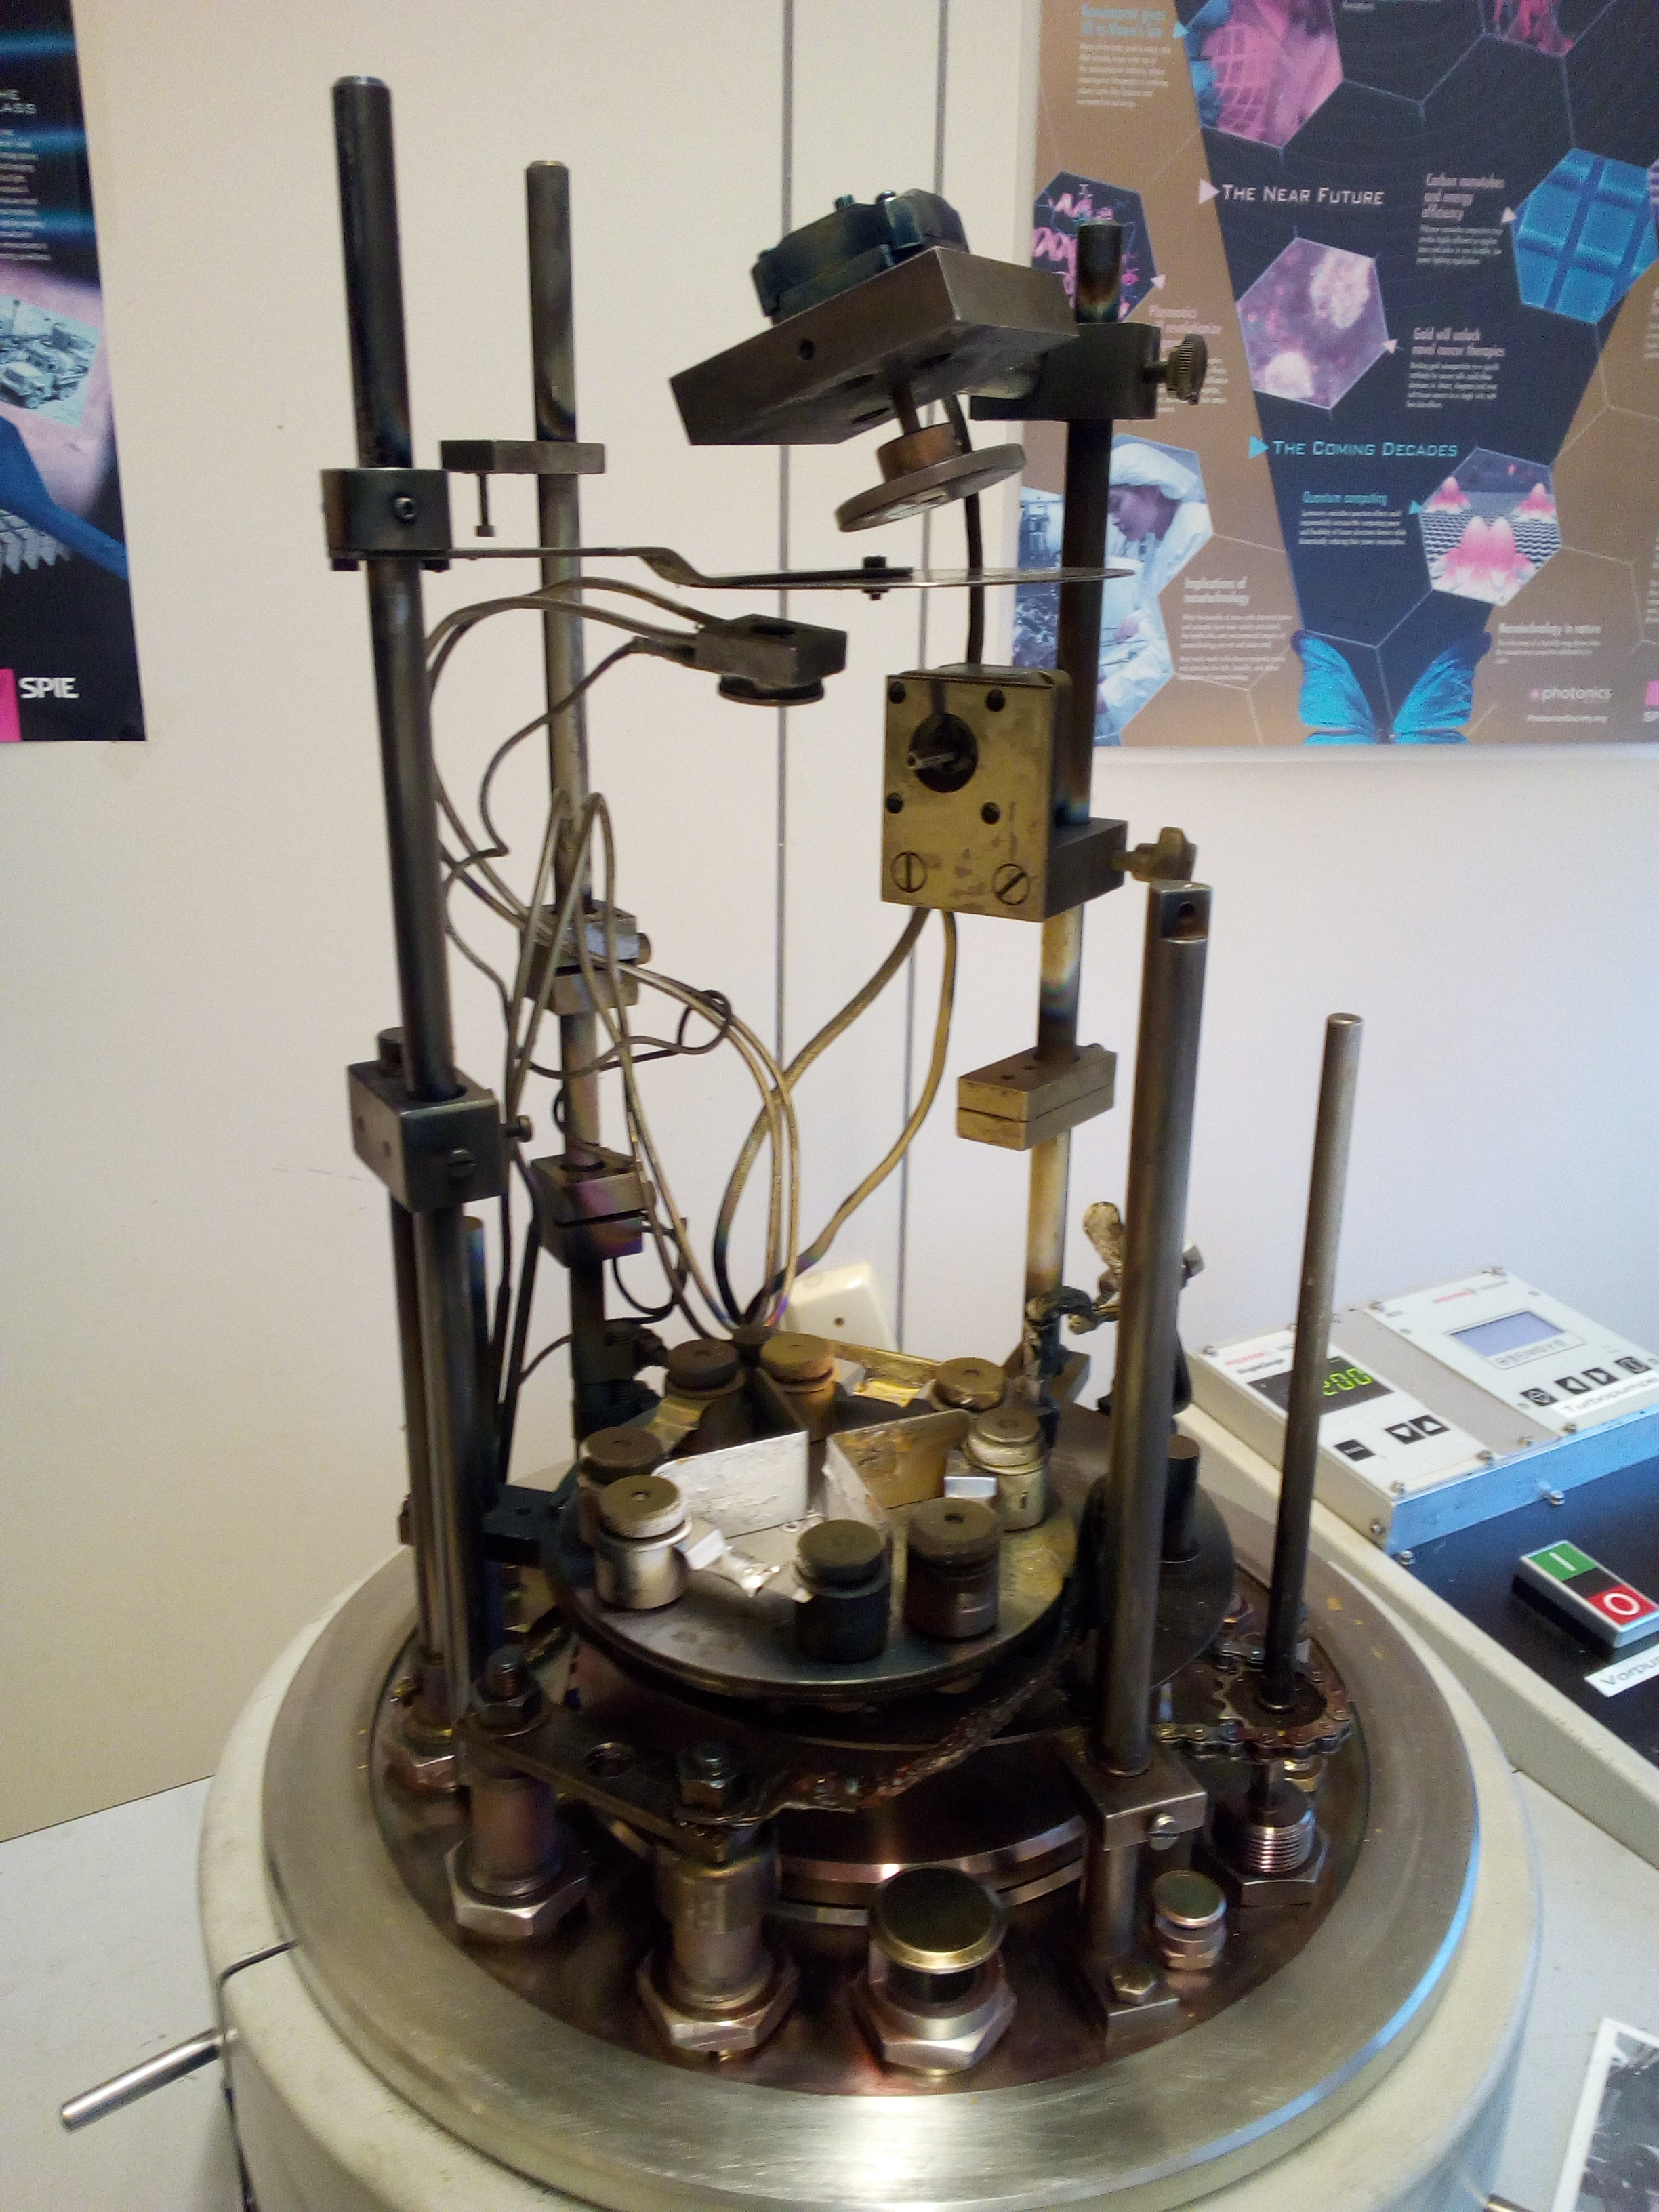
\includegraphics[width=\textwidth]{chamber.jpg}
    \subcaption{evaporation chamber}
\end{subfigure}
\end{figure}